\newpage
\chapter{Interaction in Sketch Based Software}
\label{sec:interaction}

The computational support for sketching discussed in previous sections
dealt with a wide range of topics, from hardware to data structures
and algorithms. While previous sections focused on the technology
itself, here we look more closely at people's interaction with
sketches as mediated by computational systems.

Traditional design software uses a familiar array of interaction
controls and idioms: buttons, toolbars and palettes, menus,
double-clicking and right-clicking mouse buttons, scrollbars, keyboard
shortcuts, and so on. With few exceptions, these approaches give the
user unambiguous methods to express their intentions.

However, sketching design tools must ``interpret'' user input as
messages that could have multiple meanings. If the user encircles an
object, the system must decide if this constitutes selection, or if
the circle is part of the existing object, or if the circle is part of
some other object, or if the new ink is an annotation. The semantics
of sketched user input may depend heavily on the domain as well as the
functionality the application supports.

There are several high-level classes of operations the system might
need to interpret: model, environment, and recognition/rectification
operations.

\textit{Model operations} are those marks that specify creation of new,
or modify existing, portions of the model. Some actions (such erasure)
require a target or operand, suggesting the need for sketch based
selection techniques. Freehand annotations are important for informal
work: they allow designers to record provisional ideas in
context. Such notes might be considered part of the model. If the
hardware supports it, pen properties such as pressure or angle could
be used in subtle ways to signal different kinds of input---soft marks
could indicate texture or shading, for example.

\textit{Environment operations} are messages that change the state of
the design tool itself in some way. They may specify changes in
viewing parameters such as zooming, rotating, panning, or switching
between ``rough'' and ``rectified'' renderings. Users might issue
commands for performing some task immediately, from simple requests
like printing to more involved tasks such as invoking a
simulation. Environmental commands are often issued using buttons or
menus, or they may be issued by gestures. However, interface
components designed for keyboard and mouse hardware may be
inappropriate for use in sketch based systems.

\textit{Recognition operations} allow users to initiate or interact
with a process. Some systems enable users train the recognizer by
specifying new objects or relationships among objects, which requires
training techniques. The sketching system may also let users to
trigger the recognizer rather than recognizing automatically. Some
recognition systems are non-interactive and simply use the `best'
interpretation. Other systems are interactive, enabling the user to
choose among alternatives. As with some model operations, users may be
allowed to select specific portions of their drawing for recognition.

The distinction between the above operation classes is often
blurred. For example, a gesture to erase an object (a model operation)
must be recognized before it is executed.

\section{Managing recognition error}
\label{sec:recognition-difficulties}

In any but the most trivial of tasks, sketch recognition will
occasionally fail. Either the recognizer does not correctly interpret
the user's sketch, or the recognizer is unable to produce an
interpretation. Perhaps the user's sketch was drawn in such a way that
even a human observer could not correctly interpret it. Maybe the user
drew something the recognition system was not intended to
handle. Regardless of the reason for the failure, it is important to
manage problems that arise due to failed recognition. The particular
strategy for managing error depends in part on when the system employs
recognition.

Consider an application whose recognition process assigns a numeric
confidence value describing how well a candidate entity matches
entries in the recognition library. The multiple matches are put into
an \textit{n-best list} ordered by confidence levels. When the
recognizer is obliged to report the most likely interpretation, it can
simply respond with the item with the highest confidence
value. Alternately the recognizer could respond with multiple
interpretations~\cite{gross-boe,alvarado-sketchread-uist}, but most
applications are not designed to accommodate that. Recognition results
may be inappropriate or inaccurate in a number of ways, summarized in
the following table.

\begin{table}[h]
\begin{center}
\begin{tabular}[h]{l p{8.5cm}}
Incorrect: & The user drew X but the recognizer confidently found
Y. \\

Ambiguous: & The user drew X, but the recognizer is unable to
confidently discern the possible interpretations of X, Y, or Z. \\

Uncertain: & The user drew X, but the recognizer could not confidently
find any interpretation. \\

Unintended: & The system correctly recognized X but the user was not
ready to work with recognized elements yet. \\

\end{tabular}
\label{tab:recognition-errors}
\caption{Categories of sketch recognition difficulties.}
\end{center}
\end{table}

The system may attend to inappropriate or inaccurate recognition
automatically or interactively. Interactive methods include suggestive
interfaces that provide alternative
interpretations~\cite{igarashi-suggestive}. Some systems like
BURLAP~\cite{mankoff-burlap} use both automatic as well as interactive
methods.

\section{Reacting to sketch input}
\label{sec:recognition-action}

The system must determine when and how to react once it recognizes
sketched elements. One action is to give the user feedback of
recognition results. Textual, visual, and audio feedback have been
used. Another type of action triggered by recognition is to invoke a
command or program. Finally, recognized ink may be transformed into an
interactive object whose behavior is consistent with whatever it
depicts, such as a sketched scrollbar turning into a manipulable
scrollbar~\cite{landay-silk}.

Taking action based on recognition events can be problematic because
of the inherent ambiguity and uncertainty of sketches. Passive
feedback of recognition (such as an \textit{n-best list} menu) can be
ignored. However, some forms of feedback may have lasting effects: a
sketched gesture inaccurately recognized as a delete operation can not
be easily ignored.

The Electronic Cocktail Napkin could be configured to \textit{rectify}
(and unrectify) user input but it is turned off by
default~\cite{gross-ecn-uist,gross-cocktail}. Rectification (sometimes
called \textit{beautification}) represents the user's input in a less
sketchy form, and is one method of providing visual feedback. Some
researchers feel that rectification is harmful because the input's
rough character reminds viewers the design is unfinished. Alvarado's
informal user studies of ASSIST suggests that the system should clean
up a drawing after the user finishes rather than rectifying as they
draw~\cite[page 91]{alvarado-masters-thesis}.

Beautification is not always antagonistic to design,
however. Published diagrams are usually ``cleaned up'' such that lines
are made rectilinear, or other graphic elements are made the same size
or similar spacing. Pavlidis and Van Wyk describe a system for
beautifying rough drawings after they have been
drawn~\cite{pavlidis-beautifier}. This approach calls for automatic
inference and satisfaction of graphic constraints. 

While some systems wait for users to explicitly request rectification,
Teddy renders user input as 3D shapes as they are
provided~\cite{igarashi-teddy}. Arvo and Novins demonstrate a novel
method of rectifying 2D user input while maintaining the rough,
hand-drawn qualities in the context of interactive
sketches~\cite{arvo-beautification}. The lines have a ``shape memory''
that gives them a tendency to maintain their initial visual
characteristics as users stretch, move, and bend them.

Do investigated the context and intention of hand drawn design
diagrams in order to invoke appropriate
tools~\cite{do-phd-thesis,do-design-sketches-tools}. The \textit{Right
Tool Right Time} system is based on the observation that as people
sketch, the symbols they draw might indicate the tools they need to
support their activity. For example, an architect who is thinking
about what is visible from a vantage point may draw sight lines on a
floor plan. If the sketching program recognizes the user's input as
sight lines, it could invoke a visual analysis program to show what
can be seen from the indicated point.

\section{Toolkits for sketch recognition systems}
\label{sec:recognition-toolkits}

Modern toolkits support programming of standard WIMP applications with
a standard set of widgets such as buttons, drop-down lists, and
scrollbars. These widgets are designed for use with a keyboard and
mouse, using conventional interaction idioms like double clicking and
drag-and-drop. Evidence suggests these interface widgets and
techniques are not always appropriate for sketch-based
applications~\cite{difiore-sketching-artistic,saund-inferred-mode,alvarado-skrui-guidelines}.

Microsoft's Tablet PC API supports use of a stylus in pen-aware
applications. The Tablet PC API excels at measuring and rendering user
input. It also provides methods to access various features of freehand
input such as sampling point locations, velocity, and
pressure. Plimmer and Freeman have developed InkKit, a toolkit for
building sketch recognition based interfaces using the Tablet PC
API~\cite{plimmer-inkkit}.

SATIN~\cite{hong-satin} incorporates many engineering aspects of
creating sketch-based applications including support for pen-centric
widgets like pie menus (Figure~\ref{fig:pie-menu}) or pluggable
recognizers (like Quill/gdt~\cite{long-quill-chi}). SATIN served as
the basis for applications like DENIM~\cite{lin-denim} and
SketchySPICE. However, no further applications have been built using
this toolkit. A discussion of recognizers from various points of view
(users, designers, and programmers) is presented
in~\cite{hong-recognizers}.

The CrossY system features pen-centric user interface components such
as those shown in
Figure~\ref{fig:crossy}~\cite{apitz-crossy}. High-level interaction
toolkits for sketching incorporate not only widgets, but also support
for ambiguity management and alternative recognizers. 

BURLAP's mediation strategy (see
Section \ref{sec:recognition-managing-ambiguity}) is part of the OOPS
toolkit for managing ambiguity~\cite{mankoff-oops}.

The Electronic Cocktail Napkin~\cite{gross-ecn-uist} served as a
platform for developing other tools such as \textit{Right Tool Right
Time}~\cite{do-design-sketches-tools},
\textit{Stretch-A-Sketch}~\cite{gross-stretch-a-sketch},
a Local Area Network designer~\cite{kuczun-lan-sketcher}, and
others~\cite{gross-boe}.

\section{Sketches and human-human interaction}

People use sketches to interact with other people. When we draw a map
to help somebody navigate to a location, the marks we make provide
just enough information to communicate the
route~\cite{tversky-routes}. Such maps are media for human-human
communication, and they serve their purpose well. When people make
drawings to communicate everyday, mundane information, they tend to
use consistent notation. Even when drawing to illustrate abstract
concepts (such as ``How a web search engine works'') people use a
limited visual vocabulary~\cite{hendry-sketching-explanations}.

People interact with their sketches. This goes beyond the physical act
of drawing. When we sketch, we make marks on the page, look at them,
and potentially see new meanings in our
drawing~\cite{goldschmidt-backtalk,schon-reflective}. We interact with
sketches differently depending on many factors: size of drawing
surface, kind of pen, relevant domain, expected sketch life cycle, how
public or private it is, whether we are working alone or
collaborating, and so on.

When collaborators work on problems together, they often use shared
drawing surfaces like whiteboards or big sheets of
paper. Mynatt \textit{et. al} looked at how people use whiteboards in
practice and developed the Flatland system to support those
activities~\cite{mynatt-flatland}. Marks on whiteboards are informal,
and depending on their location they may be public. Whiteboards are
used to record lists of ideas, items to buy, things to do, and so
on. They also serve as an informal record of what is going on in the
workplace. A colleague's unerased drawing may spark conversation among
others long after the sketch's original purpose has been served.

Computational whiteboard systems like Flatland,
Colab~\cite{stefik-colab}, and
Tivoli~\cite{pedersen-tivoli,moran-whiteboard} leverage the informal,
quick, semi-public properties of traditional whiteboarding
practice. At the same time, the marks on the electronic whiteboard
become interactive: lists can be sorted, items checked off; text and
drawings may be grouped, moved, scaled, rotated. Physical whiteboards
are usable only by those present; computational whiteboards may be
used by distributed teams. This functionality has been demonstrated
both by commercial collaborative conferencing tools and research
prototypes such as the Workspace Navigator~\cite{ju-navigator}.

\section{Pen interaction techniques for sketch-based systems}
\label{sec:interaction-techniques}

An important consideration for developing new technology is the
cognitive load a tool imposes~\cite{oviatt-math-quiet}. Oviatt's study
of high school mathematics students suggests that using a pen based
application on a tablet computer is significantly worse than working
problems using traditional pencil and paper. Using the tablet,
students took longer to complete math problems, and they did not like
using the technology. Anthony \textit{et. al} conducted a similar
study comparing how students write equations using different input
paradigms. The input methods included a standard WIMP interface and
freehand writing performed with a computer
stylus~\cite{anthony-multimodal}. They found that students preferred
pen input, and hand-wrote equations faster and more accurately than
using the keyboard and mouse dialog. Paper and pencil was preferred to
electronic writing, but pens of either sort are preferred over
keyboard and mouse input. Both studies support the observation that
the more attention users must allocate to using the tool, the less
attention they can give to the problem at hand.

\begin{figure}
\begin{center}
  \subfigure[Pie menu extension to the Firefox web browser.] {
    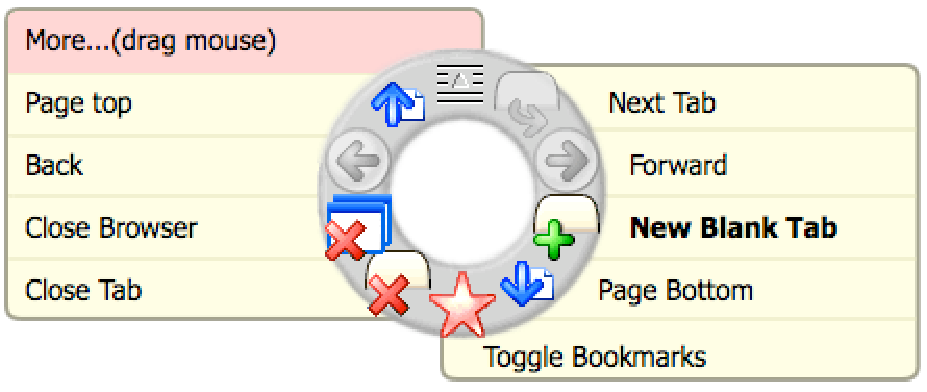
\includegraphics[angle=0, origin=c, width=2in]{img/pie-menu-browser.pdf}
    \label{fig:pie-menu-browser}
  }
  \subfigure[Autodesk Maya pie menu.] {
    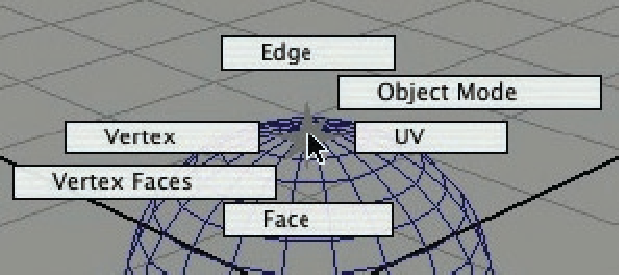
\includegraphics[angle=0, origin=c, width=2in]{img/pie-menu-maya.pdf}
    \label{fig:pie-menu-maya}
  }
  \caption{Pie menu implementations in two applications.}
  \label{fig:pie-menu}
\end{center}
\end{figure}

More natural interaction techniques must be developed in order to
reduce cognitive load. Several methods have been shown to work well
for pen applications. Marking menus are a good
example~\cite{kurtenbach-marking-menus}. Traditional menus provide a
list of options, growing downwards and to the right. For pen devices
with co-located input and output (such as a Tablet PC) the user's hand
may obscure the menu. Pie menus (a type of marking menu) appear
centered at the pointer location, with options distributed radially
(see Figure~\ref{fig:pie-menu}). The user's hand may still be
partially in the way, but at least part of the menu remains
visible. The benefit of the marking menu is that people can learn to
perform gestures without reading the option labels if the options
appear in consistent locations. The need for a visual menu eventually
disappears, leaving only the gesture. Pie menus are used in
applications such as Maya \cite{autodesk-web}, games such as the Sims
\cite{ea-sims}, and are available as add-ons to web browsers. This
approach works well, but has two drawbacks. First, it is not clear how
the menu should be invoked. Second, gestures must be discovered,
learned, and remembered.

Ramos \textit{et. al} further explored the use of pressure data for
pen based interaction~\cite{ramos-pressure-widgets}. In addition to
the stylus $(x,y)$ position, pressure serves as another dimension the
user can freely manipulate. For example, pressing lightly may produce
a menu with one set of options, while pressing hard offers a different
option set. Pressure could be effective as an input modality if used
appropriately, including haptic and visual feedback.

Traditional menus are typically invoked by clicking the mouse,
applying force orthogonal to the mouse's plane of operation, which
does not cause the mouse to move. Some computer styluses have barrel
buttons that allow users to ``right click'', but the force necessary
to depress the stylus button is liable to cause unintentional pen
movement, leading to mistakes~\cite{hinckley-input-technology}.

Hinckley \textit{et. al} suggest the use of delimiters to trigger
marking menus~\cite{hinckley-scriboli}. A delimiter is ``something
different'' in the pen input that the user is otherwise unlikely to
draw but is easy to remember. One example delimiter in their Scriboli
system is a pigtail mark, a loop made at the end of a selection
gesture. This fluid motion lets the user indicate target objects
followed by a command to apply to those objects.

Others have developed interface idioms for supporting pen and sketch
input. \textit{Gedrics} are gesture-driven icons for pen based
applications~\cite{geissler-gedrics}. Each Gedric is associated with a
class of tasks such as ``changing font properties'' in a text
editor. To invoke a command, the user draws a gesture on a Gedric. The
system recognizes the gesture, giving the icon meaning that can be
activated by tapping it. On the ``font'' Gedric, drawing a slanted
line might italicize selected text; drawing a vertical gesture from
the bottom to top increases text size. However, while Gedrics help
make some operations more convenient and reduce clutter on user
interfaces, they also require users to know how to turn their
intentions into a gesture. 

\begin{figure}
   \centering
   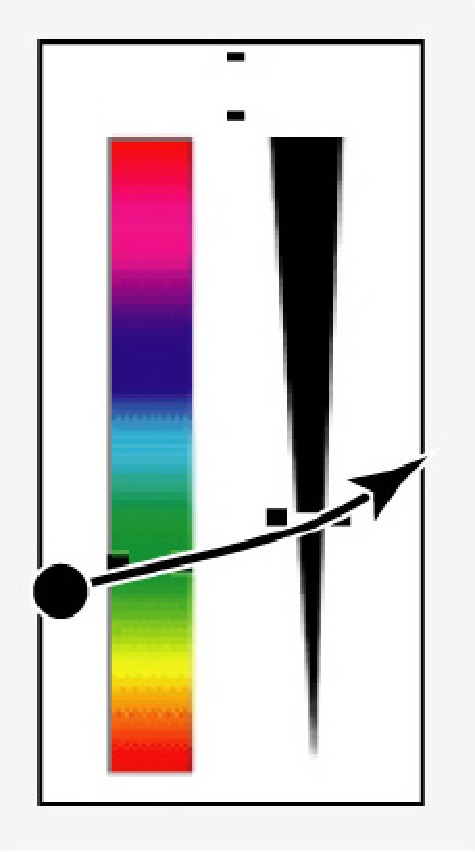
\includegraphics[width=1.2in]{img/crossy.pdf} 
   \caption{CrossY interface widgets let users change multiple
   parameters with a single stroke---pen color and thickness in
   this example.}
   \label{fig:crossy}
\end{figure}

While pointing and clicking is appropriate for tasks commonly
performed with mice, Accot and Zhai suggest ``crossing'' as an apt
technique for stylus interaction~\cite{accot-crossing}. The
experimental drawing program CrossY~\cite{apitz-crossy} demonstrates
interface widgets that support crossing. To activate a CrossY button,
the user draws a line from one side of the button to the
other. Crossing makes it easy to take multiple actions with a single
fluid motion, for example changing pen color and thickness by dragging
the pen across adjacent CrossY widgets (see Figure~\ref{fig:crossy}).

The inherent ambiguity of sketching is also present in pen based
interaction that is not intended to be sketchy, e.g. pressing a button
or choosing a menu item. When the user attempts to act on an object
the system may have to disambiguate the target. For example, when
pressing a button, the pen may accidentally slide off one into
another. This is called \textit{target
ambiguity}~\cite{mankoff-burlap,mankoff-oops}.

An alternative to mediating ambiguity is to preempt it. Pegasus and
Chateau~\cite{igarashi-pegasus,igarashi-suggestive} demonstrate a
\textit{suggestive interface} that predicts what the user will draw
and shows the outcomes of various possible actions. If a pick-list
mediator from BURLAP/OOPS is like asking you to clarify what you've
said, a suggestive interface is analogous to completing your sentence
before you finish. For example, Chateau's simplified domain of
architectural design~\cite{igarashi-suggestive} is constrained to
certain configurations of walls and beams known to produce good
results. This technique is appropriate when the domain has a highly
regular grammar or when structural properties such as symmetry may be
exploited. Tsang and colleagues use a suggestive interface for their
3D sketching system that can model shapes such as aircraft
hulls~\cite{tsang-3d-sketching}. The system provides an overlay that
guides users in providing additional sketch input. Users found this
conducive to providing precise input. The system uses the incomplete
sketch as a database query, finding similar drawings, and suggests
additional geometry that may be appropriate.

Bae's 3D curve modeling system demonstrates how several calligraphic
interaction techniques can be used together to provide a highly fluid
sketching environment~\cite{bae-ilovesketch}. The system, called
\nohyphens{ILoveSketch}, presents a physical sketchbook metaphor. Note
that like Sketchpad, input is provided using a stylus, optionally
modified by pressing physical buttons with the non-dominant hand
(Figure~\ref{fig:ilovesketch}). The interface lacks the familiar
on-screen buttons, scroll bars, and menus. Instead, users give
commands with gestures which are often context-sensitive. For example,
to browse earlier drawings the user ``peels'' back virtual pages by
dragging a corner; to erase an item the user draws a ``scratch-out''
gesture. Many techniques implemented in \nohyphens{ILoveSketch}
address challenges associated with sketching 3D objects. For example,
the system infers appropriate viewing angles by rotating or panning
based on the user's work.

\begin{figure}
   \centering
   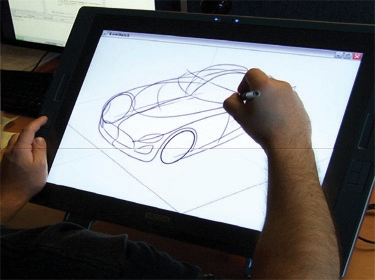
\includegraphics[width=2.5in]{img/ilovesketch.pdf} 
   \caption{ILoveSketch presents an ``as natural as possible''
     sketching system that brings together many calligraphic
     interaction techniques~\cite{bae-ilovesketch}.}
   \label{fig:ilovesketch}
\end{figure}

Alvarado provides a list of seven design guidelines for
developing \textit{Sketch Recognition User Interfaces}, or
SkRUIs~\cite{alvarado-skrui-guidelines}. These guidelines are:

\begin{small}
\begin{enumerate}
\item Display recognition results only when the user is done sketching.
\item Provide obvious indications to distinguish free sketching 
      from recognition.
\item Restrict recognition to a single domain until automatic domain 
      detection becomes feasible.
\item Incorporate pen based editing.
\item Sketching and editing should use distinct pen motions.
\item SkRUIs require large buttons.
\item The pen must always respond in real time.
\end{enumerate}
\end{small}

While WIMP interfaces have been widely used since the mid-1980s,
sketch-based interfaces remain to be adopted. To develop better
interaction guidelines, interface design patterns and toolkits, the
research community must continue to build and evaluate
sketching-centric applications.

\section{The ``mode problem''}
\label{sec:interaction-mode-problem}

User interfaces often interpret input differently depending on which
mode a program is in. For example, a structured graphics program may
have input modes such as \textit{select}, \textit{draw line},
or \textit{fill color}. Such a tool allows users to indicate
rectangular areas when the selection tool is active. The same program
also allows users to draw when the pencil tool is active. In both
cases the user presses a mouse button and drags the cursor. But the
program interprets user input in terms of the active tool. Sometimes
users are unaware of which mode the program is in, or are unsure how
to change to the desired mode. Managing modes often introduces
cognitive load by forcing users to think about the tool rather than
their work. This is called ``the mode
problem''~\cite{tesler-mode-problem}. It has been a challenge since
the beginning of interactive systems and is certainly not particular
to sketching software.

Sketchpad, arguably the first sketching system, addressed this by
letting the user control the mode with physical controls (buttons,
toggle switches, dials) with the left
hand~\cite{sutherland-sketchpad}. GRAIL users did not explicitly enter
modes to edit text and graphics. Instead, the meaning of user input
was inferred by analyzing ink and its
context~\cite{ellis-grail}. These two early systems represent opposite
extremes in ways to address the mode problem. Sketchpad's solution was
explicit mode changes using non-pen input; GRAIL's solution was
implicit mode changes done only with pen input.

There seems to be no clear ``right'' way to address the mode
problem. Implicit mode changes may seem more natural, but only if the
system correctly recognizes the user's intention. Recognition
techniques are error-prone. Many systems therefore provide a
combination of these two ways or impose drawing conventions.

Saund and Lank explored automatically recognizing mode based on the
user's input in context of what has already been
drawn~\cite{saund-inferred-mode}. Their \textit{inferred-mode
protocol} specifies an approach for analyzing the pen's trajectory and
determining if an action may be taken unambiguously. If the user's
intention is ambiguous, a mediator (such as those demonstrated by
BURLAP~\cite{mankoff-burlap}) provides the user with methods to
resolve ambiguity.

Li \textit{et. al} compared mode-switching techniques for pen based
user interfaces~\cite{li-mode-switching}. These techniques included
the pen's button, press and hold, using the non-dominant hand to press
a physical button, a novel pressure-based method, and using the eraser
end of the stylus. Interestingly, using the non-dominant hand to
switch modes was the fastest, the least error-prone, and best-liked
method. 

The ``press and hold'' approach is also used by
Schilit \textit{et. al}, who call this a ``dwell''
gesture~\cite{schilit-xlibris}.  Microsoft Windows for Tablet PCs uses
a dwell gesture for invoking right-click menus.

Scriboli's delimiters address the mode problem by allowing users to
seamlessly switch between which objects to operate on and which
commands to invoke~\cite{hinckley-scriboli}. For sketch-based systems
the mode problem arises partly because there are multiple types of pen
input. Some ink is intended to stay on the page and represents words,
pictures, or other model elements (\textit{model operations}). Other
pen input indicates selections or commands (\textit{environment
  operations}).

\begin{figure}
  \centering
  \subfigure[] {
    \label{fig:flowselection-1}
    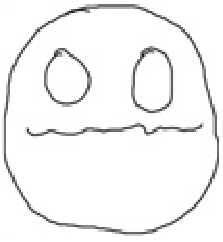
\includegraphics[origin=c,width=2.5cm]{img/flowselection-1.pdf} 
  }
  \subfigure[] {
    \label{fig:flowselection-2}
    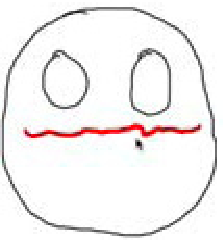
\includegraphics[width=2.5cm]{img/flowselection-2.pdf}
  }
  \subfigure[] {
    \label{fig:flowselection-3}
    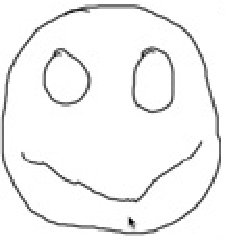
\includegraphics[origin=c,width=2.5cm]{img/flowselection-3.pdf} 
  }
  \subfigure[] { 
    \label{fig:flowselection-4}
    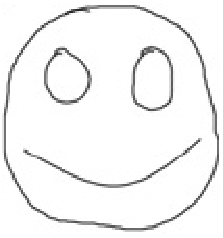
\includegraphics[origin=c,width=2.5cm]{img/flowselection-4.pdf} 
  }

  \caption{Flow selection's mode changes done by alternately holding
  and moving the stylus~\cite{johnson-flow-selection}. Here the user
  positions the stylus near the middle of the figure's mouth
  and \subref{fig:flowselection-2} moves it without lifting the
  pen \subref{fig:flowselection-3}. The user then holds the stylus
  still until the curve is smoothed \subref{fig:flowselection-4}
  before completing the process by lifting the
  pen.}  \label{fig:flow-selection}
\end{figure}


Flow selection~\cite{johnson-flow-selection} allows users to
seamlessly change modes from drawing to selecting with a dwell
gesture. Subsequent operations (such as moving part of a line) are
performed by moving the stylus without lifting up. In the example in
Figure~\ref{fig:flow-selection}, the selection strength depends on
distance to the place the user is pressing and how long the stylus has
been held down. Selection strength is then used by subsequent
operations such as moving or smoothing.

\section{Application areas of sketching}
\label{sec:interaction-application-areas}

\subsection{Problem solving}

Sketching supports everyday problem solving. A homeowner may estimate
financial figures on the back of an envelope when managing household
funds. A college student may draw a dorm room floor plan with
furniture in various configurations to determine what is possible and
desirable. Pencil and paper support these quick calculations very
well.

One problem solving domain addressed by sketching systems is
mathematics. MathPad$^{2}$~\cite{laviola-mathpad} and
MathBrush~\cite{labahn-mathbrush} let students draw pictures of
natural phenomena and relate them to equations. For example, a
physical system involving a mass on a spring can be represented with a
drawing as well as with an equation as in
Figure~\ref{fig:mathpad2}. The drawing directly communicates
qualitative aspects about the system such as location and size of
elements, while the equation governs the quantitative properties such
as the weight's mass~$m$, the spring constant~$k$ and the time
parameter's range~$t$.

\begin{figure}[h]
   \centering 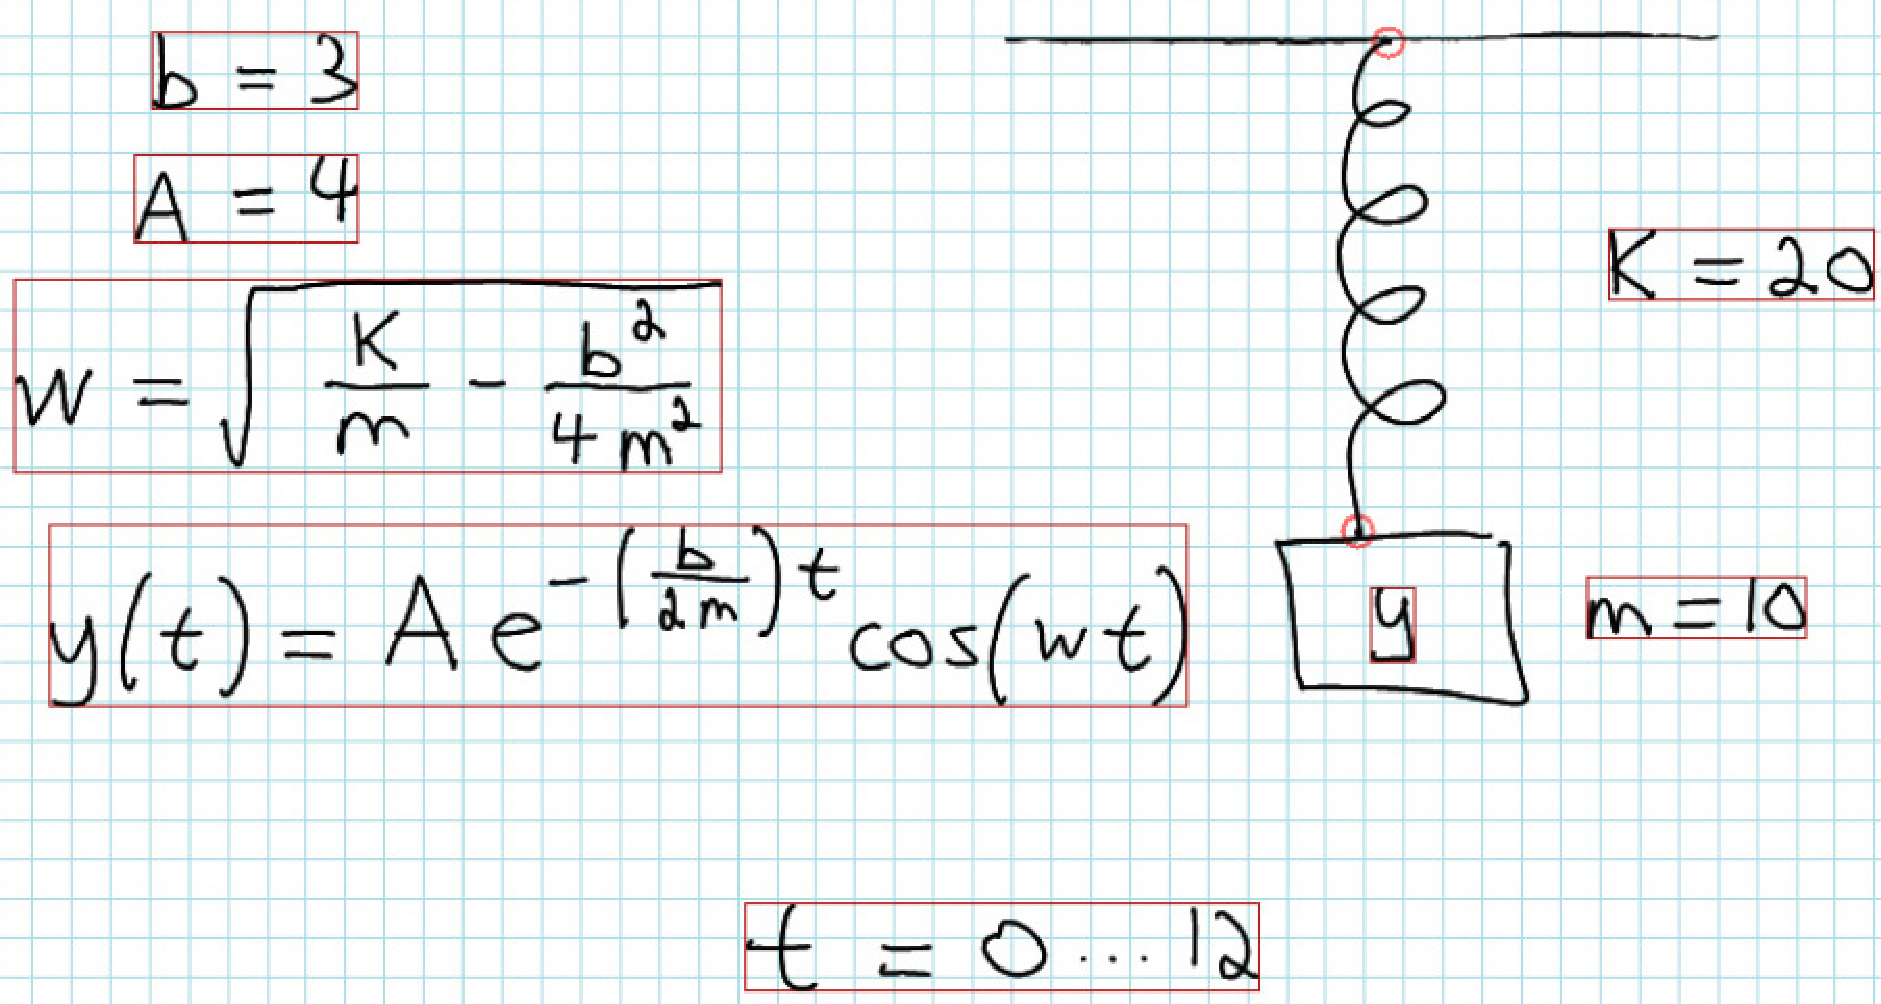
\includegraphics[width=3in]{img/mathpad2.pdf} 

   \caption{A MathPad$^{2}$ sketch showing hand-written equations
   corresponding to the drawing of the mass-and-spring system at
   right, which the system can animate.}

   \label{fig:mathpad2}
\end{figure}

Many sketching systems allow users to simulate models. The
MathPad$^{2}$ sketch in Figure~\ref{fig:mathpad2} can be set into
motion using the drawing as the initial condition, and the values $m,
k,$ and $t$ to control the animation.

Another example of problem solving addressed by sketching is editing
and annotating written documents using ink based writing or
gestures. XLibris is an electronic book that supports users in reading
documents and keeping notes on the pages, which the system
automatically organizes~\cite{schilit-xlibris}. XLibris also
recognizes certain ink commands as search requests. For example, say
an XLibris user reading this paragraph circled, underlined, or
highlighted the phrase ``electronic book''. This action silently
triggers a database query. If a strong match is found, a link appears
in the margin along with the word's definition.

\subsection{Sketch-based prototyping}
\label{sec:interaction-prototype-computer}

Sketching itself can be a form of prototyping. For example, user
interface designers often build low-fidelity paper prototypes to use
for cognitive walkthroughs or usabilty studies. The `sketchy'
appearance may facilitate brainstorming or encourage people to make
multiple interpretations of what the sketch
means~\cite{do-design-sketches-tools}. Alternately, designers may draw
to unambiguously communicate specific
designs~\cite{newman-web-designers}.

Designers draw diagrams of how components fit together in order to
better understand how to make things. At some point designers can move
past sketching and build something---a user interface, a physical
mechanism, a computer program. Before the final product is built,
several prototypes are made to help clarify the problem domain,
manufacturing constraints, usability issues, and so on. Designers
often ``go back to the drawing board'', iteratively sketching and
building prototypes.

Low-fidelity renderings of interfaces encourage discussion on the
high-level functions the UI is intended to support. Conversely,
high-fidelity prototypes encourage discussion of details that are not
important during brainstorming or early
prototyping~\cite{wong-rr-prototypes,black-fidelity}.

SILK (Sketching Interfaces Like Krazy) allows designers to draw user
interfaces and storyboards and then interact with
them~\cite{landay-silk}. SILK recognizes sketches of a limited set of
common user interface elements such as buttons, scroll bars, and text
areas. It then transforms the sketch into a high-fidelity version of
their drawn UI in the look-and-feel of their choice. The user may
elect to retain the sketchy look and still interact with the
recognized drawing. The sketch-to-prototype process is fast: users
created an interface with SILK in one fifth of the time they needed to
make the same interface with a structured interface builder.

DENIM is a system for prototyping web sites and individual page
layouts~\cite{lin-denim}. DENIM allows designers to informally and
incrementally create structures, first starting at one level of
granularity, then moving up or down as appropriate. The ability to
`zoom' from level to level is conducive to iterative web site design.

Other sketch-based systems have been developed for prototyping
computer-based models including animations with K-Sketch, multimedia
authoring with DEMAIS, and software development with
MaramaSketch~\cite{davis-k-sketch,bailey-demais,grundy-maramasketch}. These
tools allow designers to build prototypes or storyboards of dynamic
systems by creating sketches according to conventional visual
languages.

One important property of physical sketches is their ability to record
how a particular design evolved. Designers often keep journals of
drawings and refer to them for reflection. Electronic sketching
systems like SILK, ART019~\cite{yamamoto-art019}, and
NetDraw~\cite{qian-netdraw} support capturing and retrieving design
histories of drawn objects.

\subsection{Sketching 3D artifacts}
\label{sec:interaction-prototype-fab}

SILK, DENIM, and similar systems explored prototyping designs for
electronic media. Another class of sketching systems supports rapid
development of physical artifacts. Because physical objects are three
dimensional, sketching systems targeting such output frequently
involve 3D modeling.

SKETCH~\cite{zeleznik-sketch} is a 3D modeling system that
accepts gestural input to perform modeling operations, rather than a
traditional menu-based approach. The implementation described assumes
a 3-button mouse as input, but the authors suggest that pen input
would be better. The multiple buttons are used to address the mode
problem, with shape operations performed with the left mouse button
and camera operations with the right mouse button. SKETCH-N-MAKE, an
``art to part'' CAD system, added the ability to produce physical
output~\cite{bloomenthal-sketch-n-make}.

SKETCH (and SKETCH-N-MAKE) define the characteristics of the model via
a sequence of operations (extruding, cutting, etc.) on an existing
model. This approach contrasts with a freeform drawing approach
whereby designers draw shapes in 2D and the CAD system derives a three
dimensional model. The freeform approach feels more ``natural'',
approximating and augmenting pencil and paper.

Recently there has been progress in developing prototypes that
construct 3D models based on freehand 2D
sketches~\cite{lipson-correlation,masry-3d-sketch}. These systems
allow designers to directly specify shapes as they are conventionally
drawn, rather than relying on mapping gestures to modeling commands.

Rapid prototyping machinery has become affordable. This gives people
additional tools for making things. The \textit{Furniture Factory}
and \textit{Designosaur}~\cite{oh-fab} projects are ``sketch-to-fab''
systems that enable people, even children, to design simple artifacts
such as doll house furniture or dinosaur skeleton models. The
Furniture Factory recognizes the 2D sketch as adjacent orthogonal
planes, and selects appropriate jointing, leading to a CAD model
suitable for manufacture on a laser cutter. Designosaur users sketch
shapes of wooden `bones' and indicate locations for the bones to notch
together.

\section{Sketching in playful applications}

Most of the systems described above have concerned the production of
functional artifacts such as web sites, mechanisms or math
equations. We can learn a lot (even about ``serious'' interactive
systems) by building and evaluating systems that are playful.

ART019~\cite{yamamoto-art019} explores a novel sketch-based form of
interaction for artists. It provides the ability to visualize drawings
over time and easily combine model states from different moments in
the drawing's creation history. For example, an artist may select a
portion of a sketch by \textit{when} strokes were applied, rather
than \textit{where} they were applied. DiFiore and Van
Reeth~\cite{difiore-sketching-artistic} describe an interface for
artistic sketch input for an animation tool that is as fluid as
pencil-and-paper while giving animators the added ability to freely
deform and edit drawings in an artful manner.

\begin{figure}
  \centering
  \subfigure[Crayon Physics Deluxe] { 
    \label{fig:fun-crayon} 
    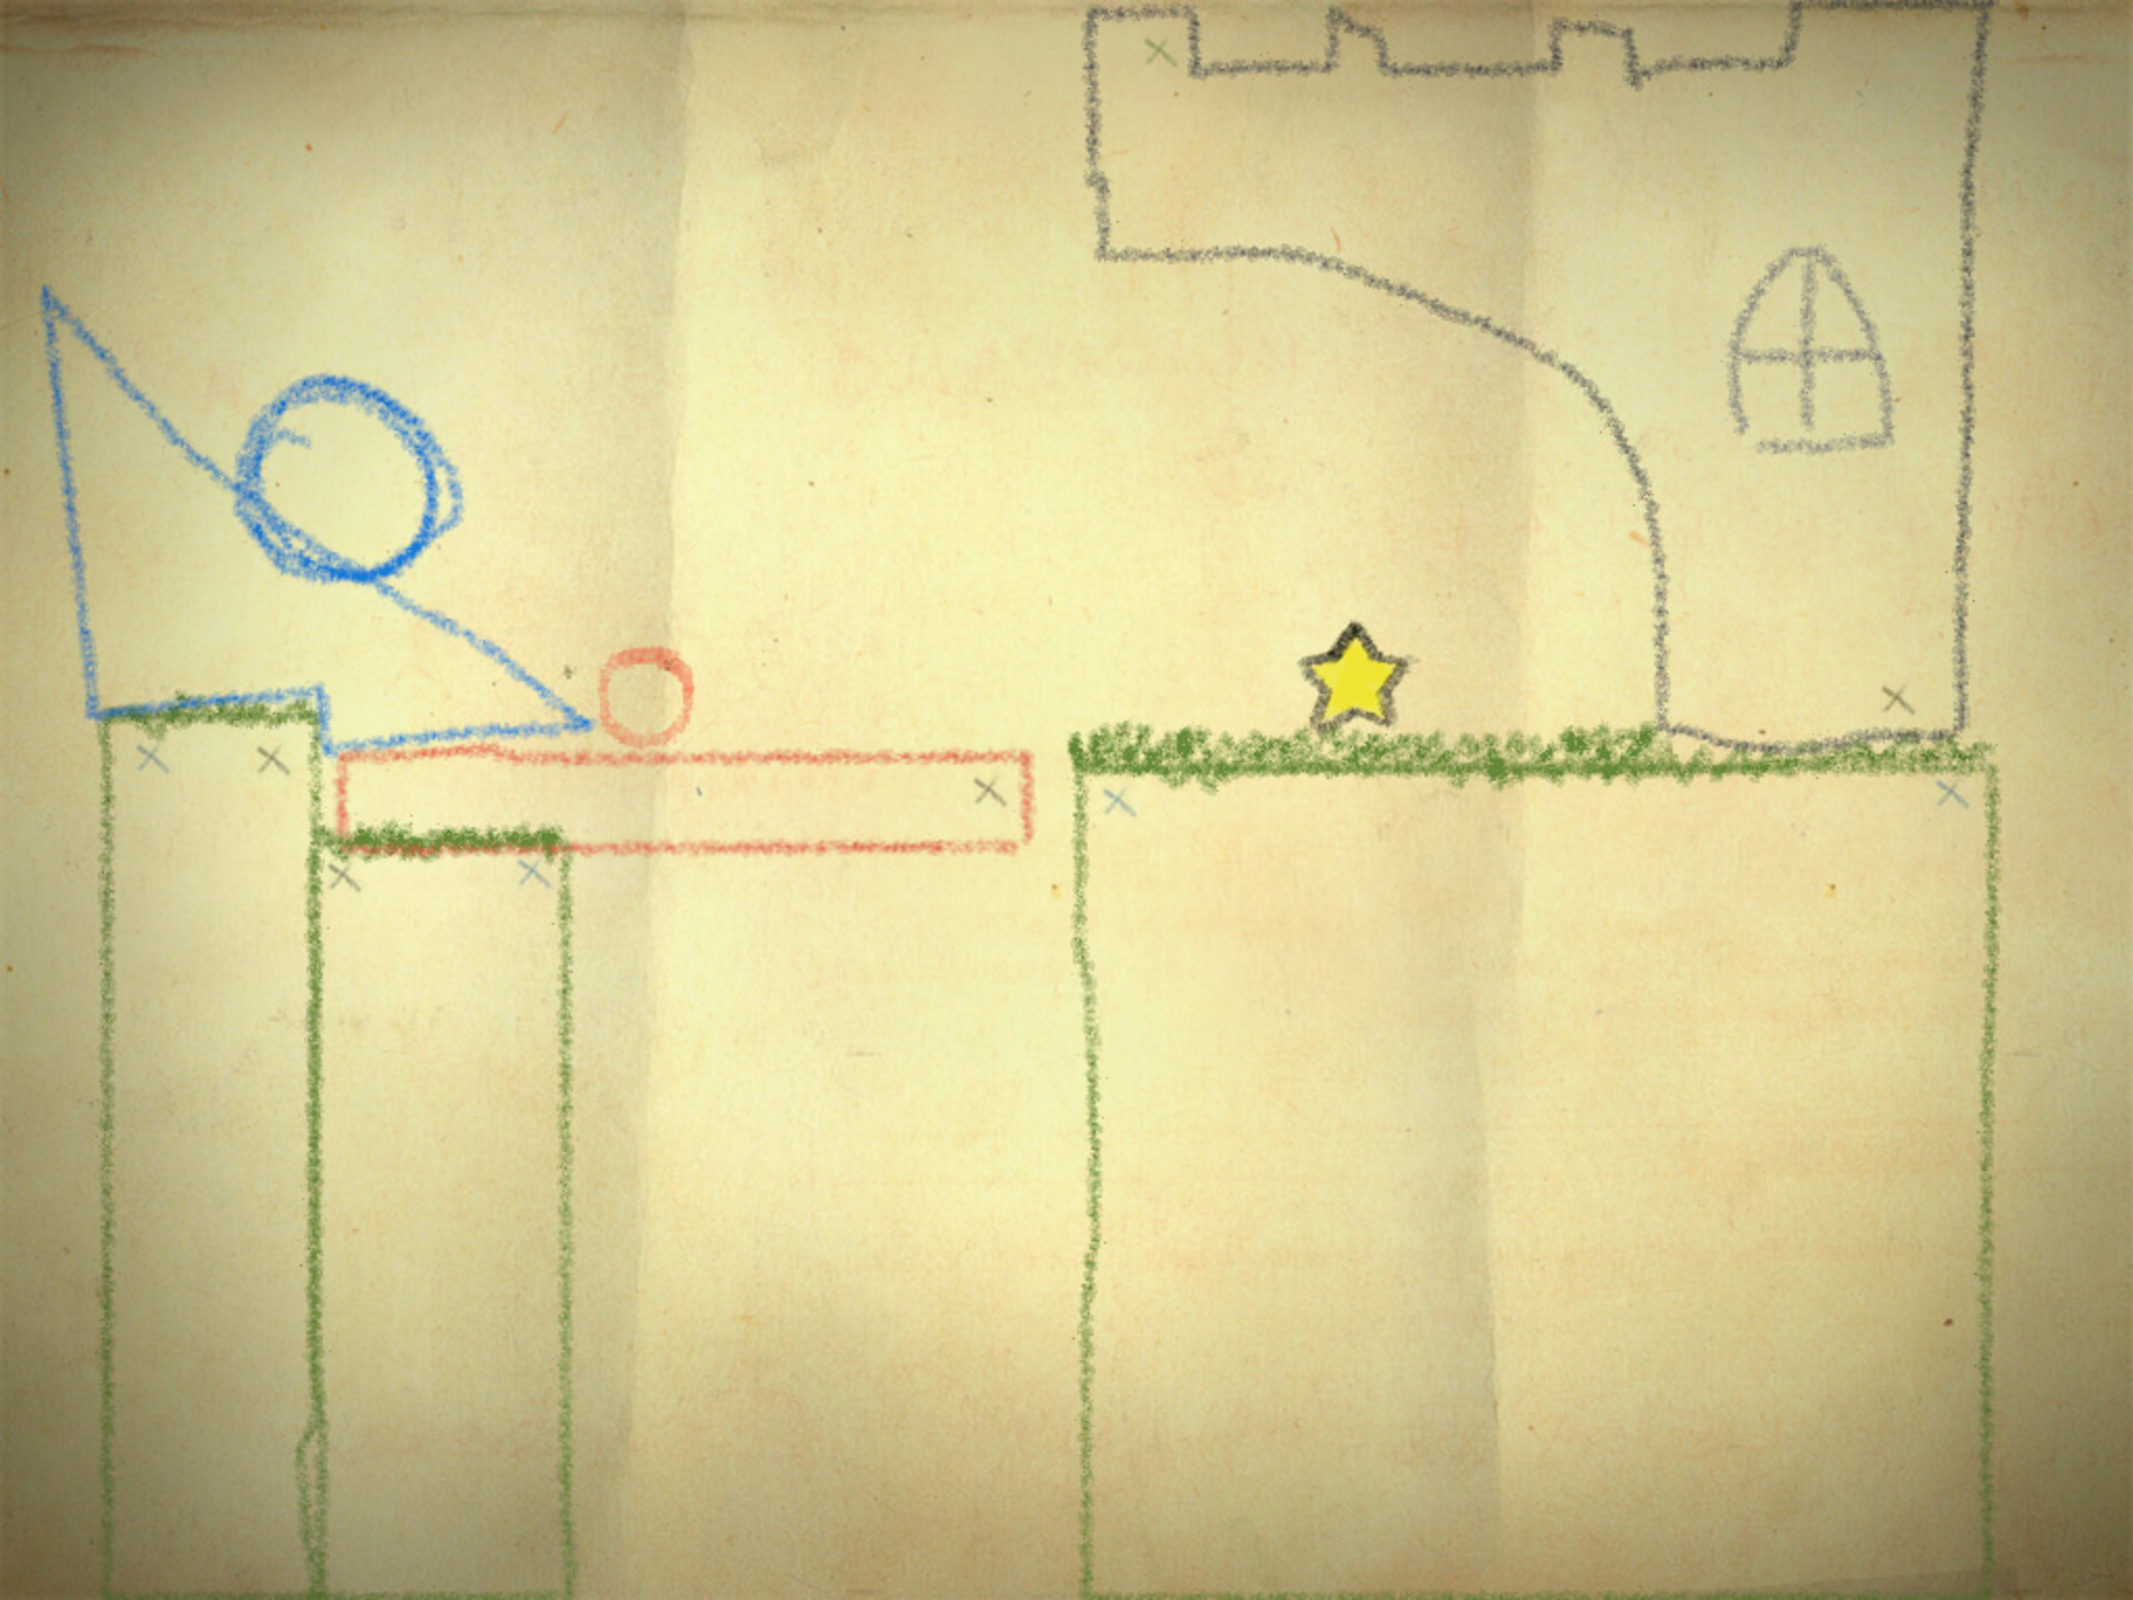
\includegraphics[width=4.5cm]{img/crayon_deluxe.pdf} 
  }
  \subfigure[Phun] {
    \label{fig:fun-phun} 
    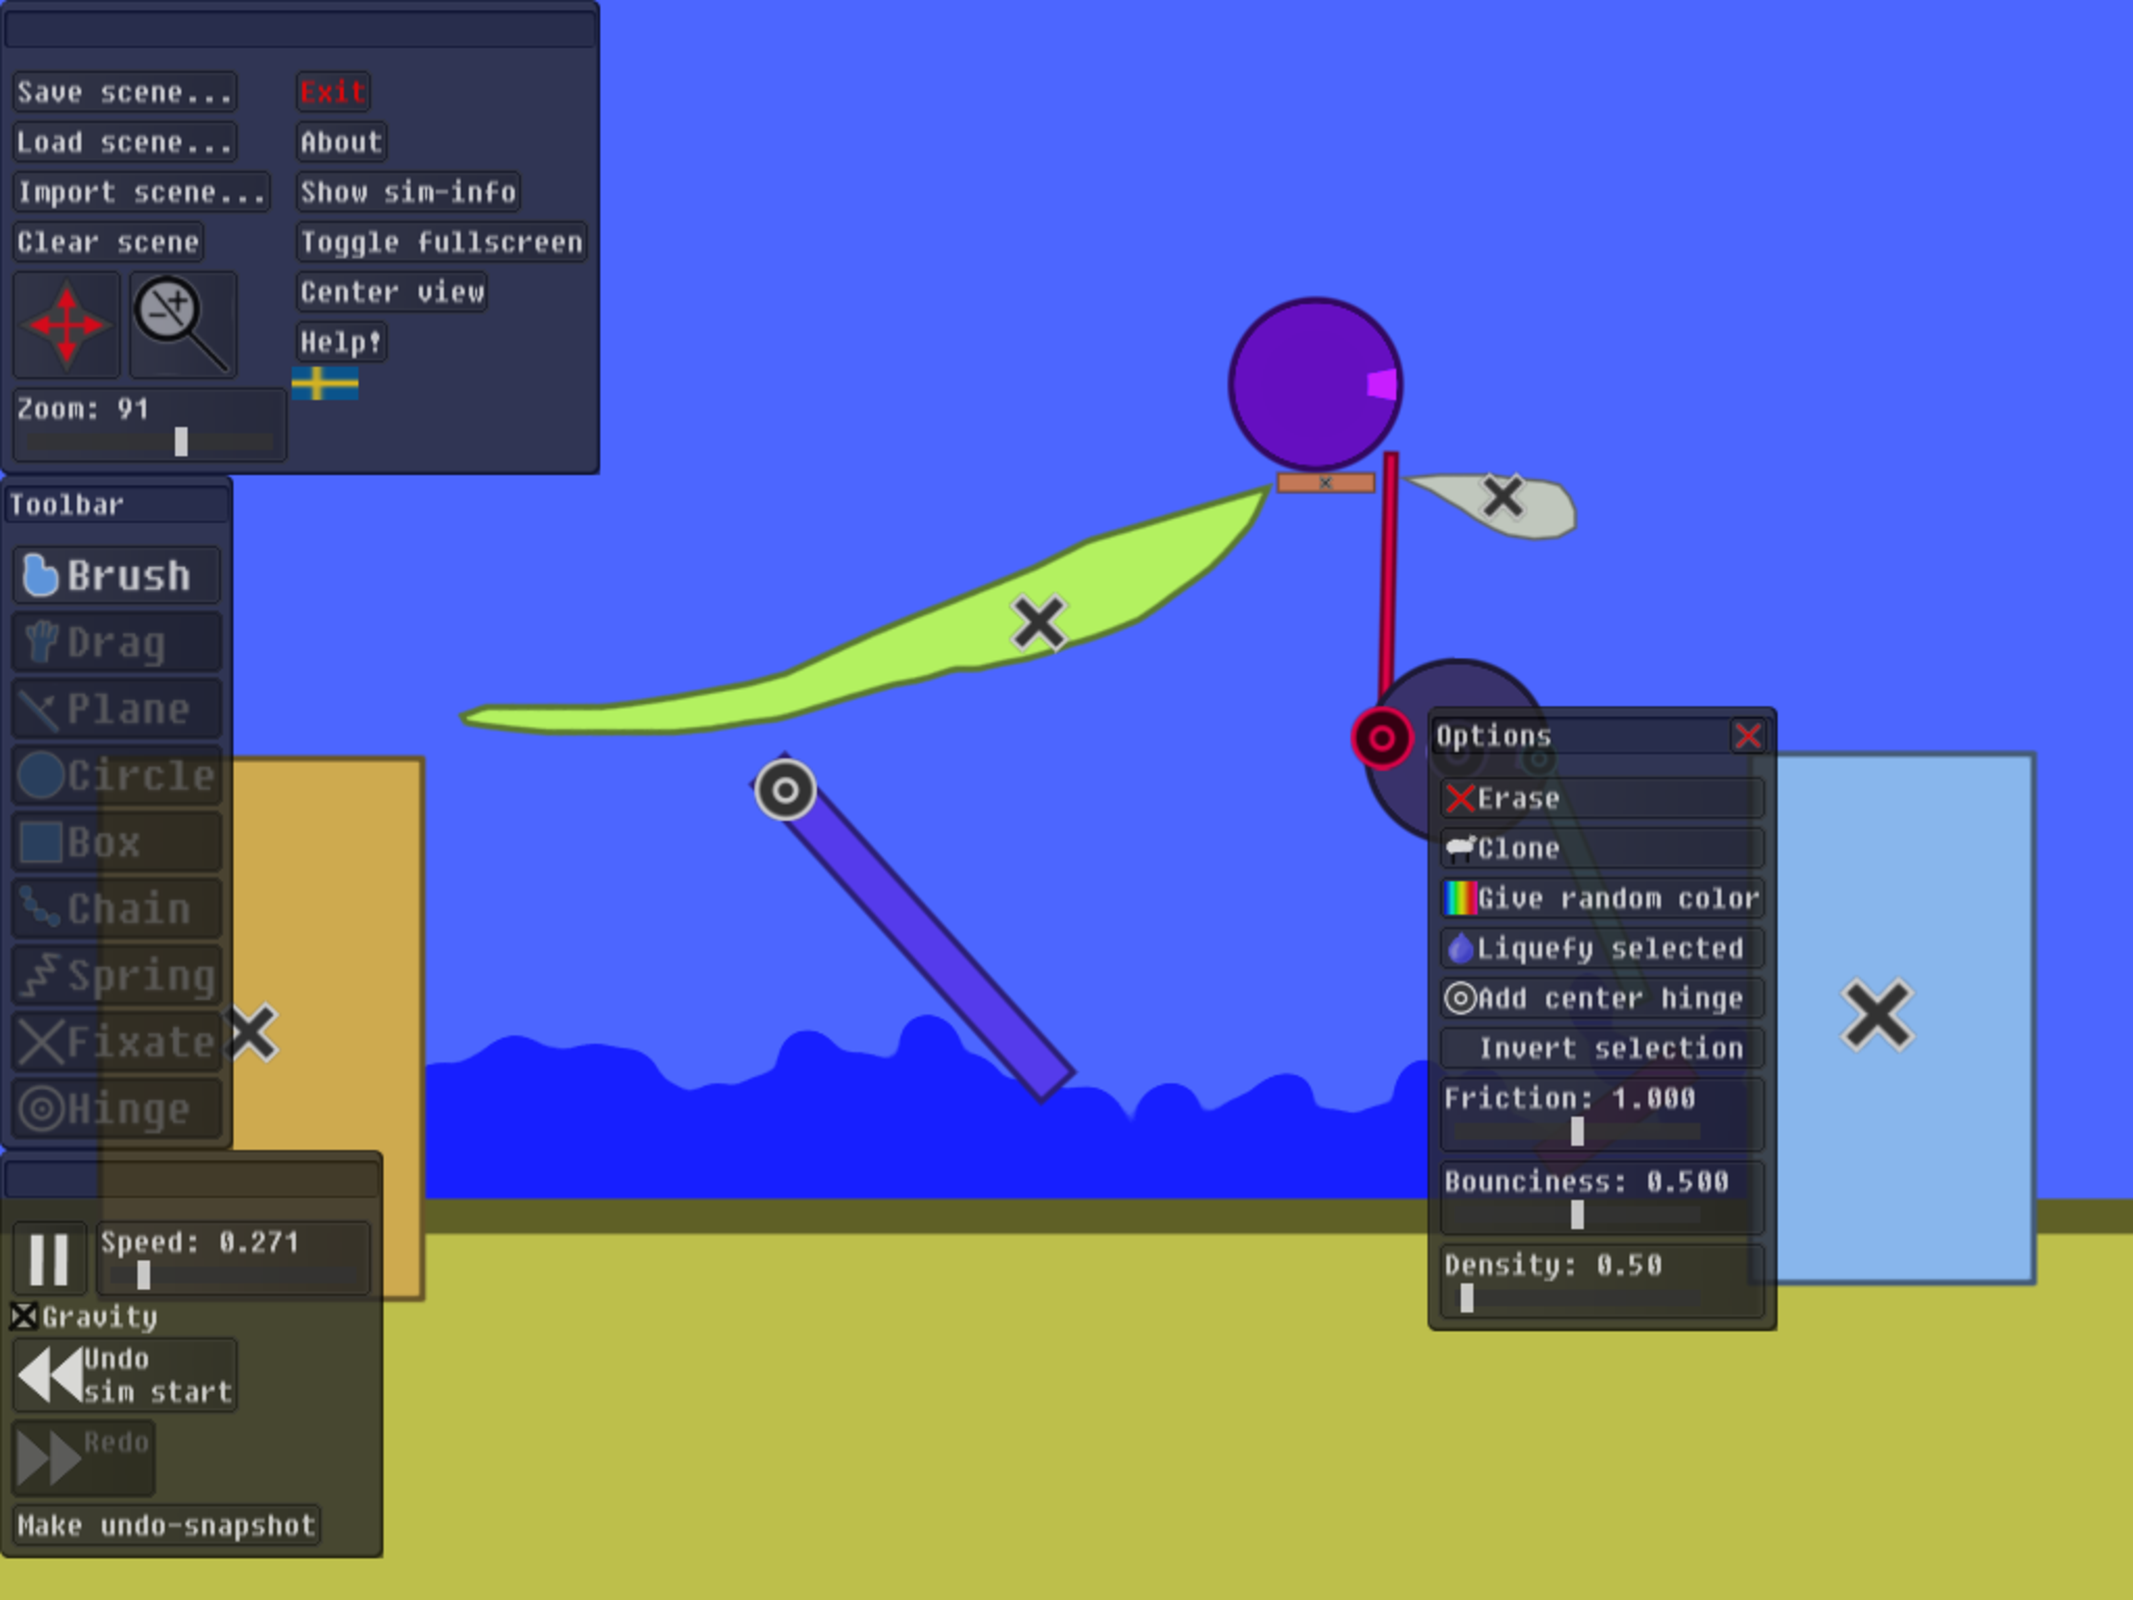
\includegraphics[width=4.5cm]{img/phun.pdf}
  }
  \caption{Two entertaining sketch-based physics simulation programs. Note the difference in how the programs render objects.}
  \label{fig:fun}
\end{figure}


Crayon Physics Deluxe and Phun are aptly-named sketching programs
wherein users draw shapes that are recognized as rigid bodies in a
physical simulation~\cite{crayon-physics-deluxe,ernerfeldt-phun}. The
user controls game play by drawing shapes that interact with one
another, subject to physical constraints such as gravity and rigid
collisions (see Figure~\ref{fig:fun}).

Paulson \textit{et. al} present a series of entertaining, educational
sketch-based systems for children to learn by
drawing~\cite{paulson-edu-sketch-games}. Their APPLES system lets
users draw elements such as planets, black holes, and arrows
representing initial velocity vectors. The recognized drawing then
becomes alive, simulating gravitational pull and elastic collisions.

Another playful calligraphic application is Plushie, a system for
designing stuffed toys~\cite{mori-plushie}. Plushie users draw shapes
that automatically turn into blobby, 3D objects rendered with
cartoon-like, non-photorealistic rendering. The system provides an
intuitive drawing environment where people can make engaging, complex
3D models.

Like Plushie, FiberMesh builds on prior work by Igarashi and
colleagues~\cite{nealen-fibermesh,igarashi-smooth}. FiberMesh enables
users to edit 3D free-form models. Users enter one of several modes
including deforming, rubbing, erasing, and type change. All strokes
remain on the model, giving the user controls for later manipulation.

The ``fun'' applications presented here provide the basis for serious
research. The act of drawing---even if it is a simple doodle---may
help to clarify the designer's
thoughts~\cite{cross-natural-intelligence}.  One participant in
Nealen's informal user study said, ``One great thing about this system is
that one can start doodling without having a specific goal in mind, as
if doodling on paper. One can just create something by drawing a
stroke, and then gradually deform it guided by serendipity, which is
very important for creative work~\cite{nealen-fibermesh}.'' 

\vspace{12pt}

This section has discussed interaction topics of computational support
for sketching. We began by presenting interaction concerning
recognition. This includes ways for handling recognition errors, and
how the system can react to sketch input and present interpretation
results to the user. Several toolkits for developing sketch based
software were presented. Application areas for supporting human
communication and design were described, with focus on areas where
sketching is particularly useful. We discussed low-level interaction
methods such as how users may select and act on objects, or how they
may explicitly or implicitly enter modes.
